\chapter{量子比特、复态矢量与可观测量}

\lectureoverview{单个电子自旋是第一个真正意义上的量子比特。它可以相对于任意空间方向进行制备，然而一个固定的探测器只返回两种结果。我们让经典磁体图像失效，然后构建描述实验实际行为所需的复矢量空间、概率规则和矩阵语言。}

\section{一个自旋与矢量的两种含义}

经典比特有两个可能状态，二者之间没有其他状态。我们可以称它们为\(0\)和\(1\)，正面和反面，或者上和下；这些名称只是经典状态空间中两个不同点的标签。量子比特在以固定方式测量时也给出两个备选结果，但它不能仅由状态空间中的两个点来描述。最简单的例子是电子的自旋。

在这个例子中有两种不同的矢量概念，将它们混淆会使后续一切变得不必要地神秘。首先是普通的\emph{空间矢量}：三维空间中的一支箭头，具有大小和方向。电子具有磁矩，就目前的目的而言，其行为如同一个小磁体。它的大小是固定的，而在制备过程中可以为其指定一个空间方向。

第二种对象是复矢量空间中的抽象矢量。这个\emph{态矢量}将描述量子态。它并不只是用另一种记号写出的磁箭头。空间方向与态矢量之间的关系是真实而重要的，但它并不是两个对象的同一性。我们将逐步获得这种关系。

\section{让经典图像失效}

有意从一个经典故事开始。将一个小磁体放入强外磁场中。除非它已经对齐，否则它会绕磁场进动。当它辐射能量时，进动逐渐阻尼，磁体最终稳定到其最低能量的取向。通过选择所施加磁场的方向、等待这种弛豫、然后撤去磁场，我们似乎能够将磁矩制备到任意期望的方向。

同一套装置提示了一种探测方法。在选定方向上开启磁场，并观察小磁体稳定过程中产生的辐射。与磁场对齐的经典磁体应当不发射能量。最初与磁场反向的磁体应当发射最大能量，而中间角度应当产生中间大小的能量。在那幅图像中，辐射能量随角度连续变化。

\begin{figure}[htbp]
\centering
\begin{coursefitfigure}
\begin{tikzpicture}[>=Latex,thick,scale=0.92]
  \draw[rounded corners] (-0.2,-0.2) rectangle (3.0,3.4);
  \node at (1.4,3.05) {\small preparation};
  \draw[->,very thick] (1.4,0.45) -- (1.4,2.55);
  \node[right] at (1.4,2.35) {\small applied field};
  \fill (1.4,1.35) circle (2.3pt);
  \draw[->,very thick] (1.4,1.35) -- (2.25,1.95);
  \node[below] at (1.4,0.15) {\small choose a direction and wait};

  \draw[->] (3.25,1.6) -- (4.25,1.6);

  \draw[rounded corners] (4.5,-0.2) rectangle (8.8,3.4);
  \node at (6.65,3.05) {\small measurement in a fixed direction};
  \draw[->,very thick] (5.15,0.45) -- (5.15,2.55);
  \fill (5.15,1.35) circle (2.3pt);
  \node[anchor=west] at (5.7,2.0) {no photon};
  \node[anchor=west] at (5.7,1.25) {one photon of fixed energy};
\node[anchor=west] at (5.7,0.5) {no intermediate outcome};
\end{tikzpicture}
\end{coursefitfigure}
\caption{操作上的困惑。连续可变的制备之后，是一个只有两种可能输出的探测器。}
\end{figure}

对于电子，那个经典预言是错误的。当探测器磁场开启时，只出现两种结果：
\begin{enumerate}
  \item 不发射光子；
  \item 发射一个光子，其能量为分隔下能级与上能级的固定能量。
\end{enumerate}
从来不会有光子携带该能量的任意分数。连续的经典响应已经坍缩为二值的量子答案。

制备中所用的方向并没有变得无关紧要。它控制着两种答案的\emph{概率}。将电子相对于探测器制备为上，则上结果确定地出现。将其制备为下，则跃迁确定地发生。将其制备为水平，则竖直探测器以相同频率返回两种答案：
\begin{equation}
  P(\text{up})=\frac12,
  \qquad
  P(\text{down})=\frac12.
  \label{eq:l02-horizontal-probabilities}
\end{equation}
因此，一个连续可变的制备族导致一个二值测量，而其统计量连续变化。

\begin{classroomqa}
\lecturetimestamp{00:21:23}
\audiencequestion{另一个小物体，也许是第二个电子，能否代替宏观磁体来提供磁场？}
\lecturerresponse{可以，但那样两个电子就构成一个联合量子系统，并且可能变得纠缠。这正是本课程将要走向的方向。我们把它推迟到单个电子的状态空间被掌握之后。}
\end{classroomqa}

\begin{classroomqa}
\lecturetimestamp{00:22:17}
\audiencequestion{概率分布是否必须通过重复整个制备和测量过程来求得？如果我们再次测量同一个电子，会发生什么？}
\lecturerresponse{是的，原始分布需要重复进行相同制备的试验。在第一次测量之后，对该电子重复同一测量会给出相同结果；该测量已将它相对于那个探测器制备好了。等待辐射跃迁本身就是一种可能的制备过程。}
\end{classroomqa}

\begin{classroomqa}
\lecturetimestamp{00:23:48}
\audiencequestion{我们设想的是一个自由电子吗，而且磁场是持续开启的吗？}
\lecturerresponse{我们分离出自旋自由度，忽略电子的位置，无论它是自由运动还是受到其他约束。一个大型电磁铁可以为了制备或探测而迅速开启。这个简化实验的设计目的只在于询问自旋。}
\end{classroomqa}

\begin{classroomqa}
\lecturetimestamp{00:25:22}
\audiencequestion{如果电子被精确制备为自旋向下，并且磁场反向，那么是否必定发射一个光子，其能量又来自何处？}
\lecturerresponse{对于精确相反的情形，跃迁以概率一发生。对于倾斜的制备，概率较小。能量最终来自建立或反转外部磁场时所做的功；装置是能量核算的一部分。}
\end{classroomqa}

\begin{classroomqa}
\lecturetimestamp{00:27:31}
\audiencequestion{光子何时出现？跃迁是瞬时的吗？}
\lecturerresponse{发射时间是随机的，就像不稳定态的衰变时间一样。可以指定一个特征寿命或半衰期，而更强的磁场会缩短这一尺度。能量--时间不确定性进入更精细的描述，但当前的操作性事实是两个可能的输出及其测量到的频率。}
\end{classroomqa}

\begin{classroomqa}
\lecturetimestamp{00:29:17}
\audiencequestion{一束包含一百万个相同制备的电子的束流，是否只会产生一个可测量的光强？}
\lecturerresponse{是的。系综强度揭示了平均跃迁概率，而任何特定电子的发射时间仍然是随机的。系综展示了单次试验无法展示的分布。}
\end{classroomqa}

这就是出发点。两个孤立的经典点可以编码探测器的答案，但它们无法编码所有改变这些答案概率的制备。我们需要一个不同的态空间。

\section{复数与态空间的几何}

所需的态空间是线性的：其元素可以相加，也可以乘以标量。其标量是复数。写
\begin{equation}
  z=a+ib,
  \qquad
  i^2=-1,
  \qquad
  z^*=a-ib,
  \label{eq:l02-complex-number}
\end{equation}
其中 \(a\) 和 \(b\) 是实数。复共轭产生正量
\begin{align}
  z^*z
  &=(a-ib)(a+ib) \notag\\
  &=a^2+b^2.
  \label{eq:l02-complex-norm}
\end{align}
这一简单的相消是概率法则的代数种子。

\begin{figure}[htbp]
\centering
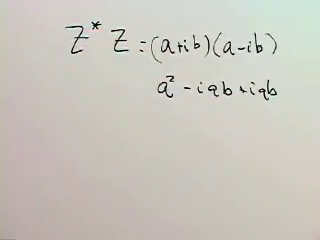
\includegraphics[width=0.74\linewidth]{lecture_02_figure_02.png}
\caption{在振幅被解释为概率之前，复共轭和 \(z^*z\) 已在黑板上展开。}
\lectureframe{00:37:10}
\end{figure}

一个复向量空间包含对象 \(\ket a,\ket b,\ldots\)，对于它们，只要 \(c\) 是复数，
\begin{equation}
  c\ket a,
  \qquad
  \ket a+\ket b
\end{equation}
就仍然是向量。列向量给出一个具体的实现：
\begin{equation}
  \begin{aligned}
    \ket a&=
    \begin{pmatrix}
      a_1\\a_2\\ \vdots\\a_n
    \end{pmatrix},
    &
    c\ket a&=
    \begin{pmatrix}
      ca_1\\ca_2\\ \vdots\\ca_n
    \end{pmatrix},\\[0.7em]
    \ket a+\ket b&=
    \begin{pmatrix}
      a_1+b_1\\a_2+b_2\\ \vdots\\a_n+b_n
    \end{pmatrix}.
  \end{aligned}
  \label{eq:l02-vector-operations}
\end{equation}
甚至复数本身也构成一个一维复向量空间。对于电子自旋，我们将需要两个维度。

对每个列右矢，我们关联一个共轭行左矢：
\begin{equation}
  \ket a=
  \begin{pmatrix}a_1\\a_2\end{pmatrix}
  \quad\longleftrightarrow\quad
  \bra a=
  \begin{pmatrix}a_1^*&a_2^*\end{pmatrix}.
  \label{eq:l02-bra-ket-components}
\end{equation}
内积则为
\begin{equation}
  \braket{b}{a}=b_1^*a_1+b_2^*a_2,
  \label{eq:l02-inner-product}
\end{equation}
而模平方为
\begin{equation}
  \braket{a}{a}=|a_1|^2+|a_2|^2.
  \label{eq:l02-norm}
\end{equation}
它是实数且非负，因为每一项都具有 \(z^*z\) 的形式。

\begin{classroomqa}
\lecturetimestamp{00:45:24}
\audiencequestion{为什么左矢符号上没有显式的星号？}
\lecturerresponse{将右矢变为其左矢已经意味着转置和复共轭。括号的反转就是该运算的记号，因此再写一个星号会重复已经隐含的内容。}
\end{classroomqa}

\section{量子比特基与玻恩定则}

现在回到探测器。令 \(\ket{+}\) 表示其向上态，\(\ket{-}\) 表示其向下态。一般的自旋态是线性组合
\begin{equation}
  \ket\psi=a_+\ket{+}+a_-\ket{-}
  \quad\longleftrightarrow\quad
  \begin{pmatrix}a_+\\a_-\end{pmatrix}.
  \label{eq:l02-general-qubit}
\end{equation}
右矢内部的加号和减号是标签，不是算术运算。一旦选定了这个有序基，
\begin{equation}
  \ket{+}=
  \begin{pmatrix}1\\0\end{pmatrix},
  \qquad
  \ket{-}=
  \begin{pmatrix}0\\1\end{pmatrix}.
  \label{eq:l02-basis-columns}
\end{equation}
确实，
\begin{equation}
  a_+\begin{pmatrix}1\\0\end{pmatrix}
  +a_-\begin{pmatrix}0\\1\end{pmatrix}
  =
  \begin{pmatrix}a_+\\a_-\end{pmatrix}.
  \label{eq:l02-basis-expansion}
\end{equation}

\begin{figure}[htbp]
\centering
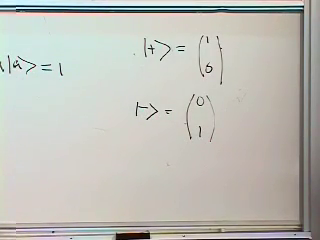
\includegraphics[width=0.72\linewidth]{lecture_02_figure_03.png}
\caption{探测器态被固定为两个标准基列。}
\lectureframe{00:58:10}
\end{figure}

这些系数是概率振幅。每个探测器结果的概率是相应振幅的模平方：
\begin{equation}
  P(+)=|a_+|^2,
  \qquad
  P(-)=|a_-|^2.
  \label{eq:l02-born-rule}
\end{equation}
由于这些是仅有的结果，
\begin{equation}
  \begin{gathered}
    |a_+|^2+|a_-|^2=1,\\
    \text{or equivalently}\qquad \braket{\psi}{\psi}=1.
  \end{gathered}
  \label{eq:l02-normalization}
\end{equation}
因此物理态矢量是归一化的。

\begin{classroomqa}
\lecturetimestamp{00:56:54}
\audiencequestion{加号和减号在分量中具有代数意义吗？}
\lecturerresponse{在这里，它们标记两个基态及其系数。我们可以称它们为 \(1\) 和 \(2\)，或者向上和向下。特别地，\(-\ket{+}\) 是 \(\ket{+}\) 的一个有效标量倍数；它不是态 \(\ket{-}\)。}
\end{classroomqa}

将态乘以一个模为1的复数，其所有概率保持不变：
\begin{equation}
  \ket\psi\longmapsto e^{i\phi}\ket\psi,
  \qquad
  |e^{i\phi}a_\pm|^2=|a_\pm|^2.
  \label{eq:l02-global-phase}
\end{equation}
因此，仅相差一个整体相位的两个矢量表示同一个物理态。\emph{相对}相位则不同。例如，仅将\(a_-\)替换为\(-a_-\)，一般不能通过将整个矢量乘以一个相位来消除；它可能改变在另一组基下测量的结果。

\begin{classroomqa}
\lecturetimestamp{00:59:54}
\audiencequestion{\(\ket{+}\)、\(-\ket{+}\)和\(e^{i\phi}\ket{+}\)是不同的态吗？改变叠加中某一项的符号又如何？}
\lecturerresponse{它们是不同的数学矢量，但当该因子乘以整个矢量且模为1时，它们描述同一个物理态。上、下两项之间的相对符号或相位在适当的测量中是可观测的，因此会改变态。}
\end{classroomqa}

该基是正交归一的：
\begin{align}
  \braket{+}{+}&=1,
  &\braket{-}{-}&=1,
  \notag\\
  \braket{+}{-}&=0,
  &\braket{-}{+}&=0.
  \label{eq:l02-orthonormality}
\end{align}
例如，
\begin{equation}
  \braket{+}{-}
  =
  \begin{pmatrix}1&0\end{pmatrix}
  \begin{pmatrix}0\\1\end{pmatrix}
  =0.
\end{equation}

\begin{figure}[htbp]
\centering
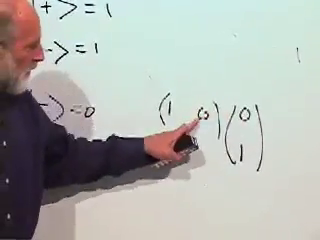
\includegraphics[width=0.76\linewidth]{lecture_02_figure_04.png}
\caption{上/下基的四个内积直接在黑板上逐一验证。}
\lectureframe{01:05:00}
\end{figure}

等权重态在黑板上给出了第一个有用的修正。列
\begin{equation}
  \begin{pmatrix}1\\1\end{pmatrix}
\end{equation}
的模平方为\(2\)，而不是\(1\)，因此未归一化。除以\(\sqrt2\)即可修正：
\begin{equation}
  \ket{\rightarrow}
  =
  \frac{1}{\sqrt2}
  \begin{pmatrix}1\\1\end{pmatrix}
  =
  \frac{\ket{+}+\ket{-}}{\sqrt2}.
  \label{eq:l02-horizontal-state}
\end{equation}
它在竖直探测器中给出\(P(+)=P(-)=1/2\)，并对应于一次水平制备。从\((1,1)^T\)到\(2^{-1/2}(1,1)^T\)的修正并非表面修饰：正是归一化把振幅平方变成完整的概率分布。

课间休息后，值得回到矢量的两种含义。空间箭头有三个实分量。量子比特态矢量有两个复分量，因此在施加归一化和认同整体相位之前有四个实数。这些对象彼此相关，但其中一个并非只是另一个的重新标记。我们目前还不需要它们之间完整的几何映射。

\begin{classroomqa}
\lecturetimestamp{01:10:56}
\audiencequestion{我们如何知道另一个量子系统的态空间的维数？}
\lecturerresponse{实验告诉我们，一次完备测量能够区分多少个互斥结果。电子自旋有两个这样的结果，因此有一个二维复态空间。自旋为1的系统在相应测量中有三个结果，因此需要三个分量。}
\end{classroomqa}

\section{经典可观测量与系综平均}

描述了态之后，转向可测量的量。在一个具有离散态\(n\)的经典系统中，可观测量是这些态上的实值函数\(f_n\)。如果态不确定并由概率\(p_n\)描述，其系综平均为
\begin{equation}
  \langle f\rangle_{\mathrm{ens}}
  =\sum_n p_n f_n.
  \label{eq:l02-classical-expectation}
\end{equation}
该记号并不意味着单次测量必须等于这个数。

对于一枚硬币，指定\(f_+=+1\)和\(f_-=-1\)。于是
\begin{equation}
  \langle f\rangle_{\mathrm{ens}}
  =p_+-p_-.
  \label{eq:l02-coin-expectation}
\end{equation}
公平硬币的平均值为零。如果\(p_+=3/4\)且\(p_-=1/4\)，平均值为\(1/2\)。\(0\)和\(1/2\)都不是单次抛掷的结果；它们各自概括了许多\(+1\)和\(-1\)的结果。

\begin{classroomqa}
\lecturetimestamp{01:23:30}
\audiencequestion{当两个值都不可能出现在单次试验中时，期望值怎么会是零或二分之一？}
\lecturerresponse{“期望值”这个说法可能引起误解。它指的是大系综的平均，而不是下一次运行中应当看到的值。公平的\(+1\)和\(-1\)结果序列平均为零，而三比一的不平衡平均为二分之一。}
\end{classroomqa}

一个特别有用的可观测量是某个态的指示函数：
\begin{equation}
  \chi_k(n)=
  \begin{cases}
    1,&n=k,\\
    0,&n\ne k.
  \end{cases}
\end{equation}
其平均为
\begin{equation}
  \langle\chi_k\rangle_{\mathrm{ens}}=p_k.
\end{equation}
因此，知道所有经典可观测量的平均值，特别地也就包含了知道概率分布。

\section{矩阵与量子可观测量}

在量子力学中，可观测量不是由态空间点上的函数表示，而是由线性算子表示。在有限维态空间中，这些算子就是矩阵。矩阵\(M\)将一个矢量映射为另一个矢量：
\begin{equation}
  M\ket a=\ket{a'}.
  \label{eq:l02-matrix-action}
\end{equation}
对于两个分量，
\begin{equation}
  \begin{pmatrix}
    m_{11}&m_{12}\\
    m_{21}&m_{22}
  \end{pmatrix}
  \begin{pmatrix}a_1\\a_2\end{pmatrix}
  =
  \begin{pmatrix}
    m_{11}a_1+m_{12}a_2\\
    m_{21}a_1+m_{22}a_2
  \end{pmatrix}.
  \label{eq:l02-matrix-components}
\end{equation}

\begin{figure}[htbp]
\centering
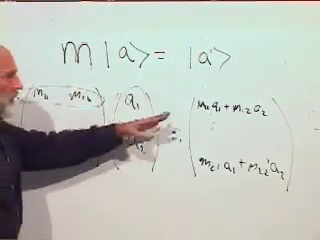
\includegraphics[width=0.78\linewidth]{lecture_02_figure_05.png}
\caption{矩阵作用逐行展开为变换后矢量的两个分量。}
\lectureframe{01:32:10}
\end{figure}

实二维向量使几何直观可见。矩阵
\begin{equation}
  \begin{pmatrix}2&0\\0&2\end{pmatrix},
  \qquad
  \begin{pmatrix}1&0\\0&2\end{pmatrix},
  \qquad
  \begin{pmatrix}2&0\\0&1\end{pmatrix}
\end{equation}
分别将每个方向均匀拉伸、只拉伸\(y\)分量、只拉伸\(x\)分量。矩阵
\begin{equation}
  \begin{pmatrix}0&1\\1&0\end{pmatrix}
\end{equation}
交换两个分量，并将平面关于\(x=y\)反射。与此同时，
\begin{equation}
  \begin{pmatrix}0&1\\-1&0\end{pmatrix}
  \begin{pmatrix}v_x\\v_y\end{pmatrix}
  =
  \begin{pmatrix}v_y\\-v_x\end{pmatrix}
  \label{eq:l02-quarter-turn}
\end{equation}
按照板书所用的约定，将向量顺时针旋转四分之一圈。剪切变换提供了另一个线性例子，不过其矩阵留作练习。本质性的限制在于线性：并非平面上每一种可以想象的变换都能用矩阵表示。

量子可观测量属于一个特殊的类。

\begin{definition}
矩阵 \(M\) 是 \emph{Hermitian} 的，当
\begin{equation}
  M_{ij}=M_{ji}^*.
  \label{eq:l02-hermitian-condition}
\end{equation}
\end{definition}

对角条件\(M_{ii}=M_{ii}^*\)迫使每个对角元为实数。非对角元以共轭对的形式出现。例如，
\begin{equation}
  M=
  \begin{pmatrix}
    r&4+i\\
    4-i&s
  \end{pmatrix},
  \qquad r,s\in\mathbb R,
  \label{eq:l02-hermitian-example}
\end{equation}
是厄米的。如果所有元素恰好都是实数，那么厄米与对称是一回事。

\begin{figure}[htbp]
\centering
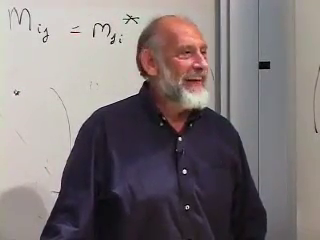
\includegraphics[width=0.75\linewidth]{lecture_02_figure_06.png}
\caption{定义性的沿对角线共轭，\(M_{ij}=M_{ji}^*\)，被单独放在本讲末尾。}
\lectureframe{01:42:50}
\end{figure}

厄米矩阵将表示可测量的量，包括沿\(x\)、\(y\)和\(z\)方向的自旋。不应把它们与描述物理踢击或时间演化的算符相混淆。

\begin{classroomqa}
\lecturetimestamp{01:45:49}
\audiencequestion{如果一个矩阵把态踢到另一个态，它是否必须保持归一化？厄米矩阵会做到这一点吗？}
\lecturerresponse{物理踢击必须保持态向量的长度，但一般的厄米矩阵并不如此。保持长度的变换是酉变换。厄米算符表示可观测量；酉算符表示作用于态的可逆变换。它们之间的详细关系接下来给出。}
\end{classroomqa}

我们已经达到了下一步所需的最低限度的语言。量子比特是二维复向量空间中的归一化向量；振幅决定概率；可观测量是厄米矩阵。有了这些部件，就可以讨论沿任意方向的自旋，并最终讨论纠缠对，而不必回到已经失败的经典图像。